\begin{table}[h]
\centering
\resizebox{\textwidth}{!}{%
\begin{tabular}{rllll}
\hline
Variable & Description & Mean & Standard Dev. & Units \\ \hline
U850 & Zonal wind at 850 mbar pressure surface & 1.56 & 8.29 & m/s \\
V850 & Meridional wind at 850 mbar pressure surface & 0.270 & 6.22 & m/s \\
UBOT & Lowest level zonal wind & 0.129 & 6.65 & m/s \\
VBOT & Lowest model level meridional wind & 0.332 & 5.77 & m/s \\
TS & Surface temperature (radiative) & 271 & 23.7 & K \\
T200 & Temperature at 200 mbar pressure surface & 213 & 7.99 & K \\
T500 & Temperature at 500 mbar pressure surface & 253 & 12.8 & K \\
TREFHT & Reference height temperature & 279 & 22.5 & K \\
TMQ & Total (vertically integrated) precipitable water & 19.3 & 15.8 & kg/m$^{2}$ \\
QREFHT & Reference height humidity & 7.83 $\times$ 10$^{-3}$ & 6.20 $\times$ 10$^{-3}$ & kg/kg \\
PRECT & Total (convective and large-scale) precipitation rate (liq + ice) & 2.95 $\times$ 10$^{-8}$ & 1.56 $\times$ 10$^{-7}$ & m/s \\
ZBOT & Lowest model level height & 61.3 & 4.91 & m \\
Z200 & Geopotential Z at 200 mbar pressure surface & 11.7 $\times$ 10$^{3}$ & 0.635 $\times$ 10$^{3}$ & m \\
Z1000 & Geopotential Z at 1000 mbar pressure surface & 474 & 833 & m \\
PS & Surface pressure & 96.6 $\times$ 10$^{3}$ & 9.71 $\times$ 10$^{3}$ & Pa \\
PSL & Sea level pressure & 101 $\times$ 10$^{3}$ & 1.46 $\times$ 10$^{3}$ & Pa \\ \hline
\end{tabular}%
}
\caption{Atmospheric variables contained in the ClimateNet dataset \cite{prabhat2020climatenet, radke2024explaining}.}
\label{tab:variables}
\end{table}

ClimateNet is a community-sourced, expert-labeled open dataset designed to bridge the gap between deep learning and climate science. It was developed to address the lack of high-quality, labeled data for training machine learning models to identify and track extreme weather events. Traditionally, climate scientists used heuristics to identify storms. These rules are often inconsistent. ClimateNet provides ground-truth labels created by human experts, allowing researchers to train segmentation models. The ClimateNet dataset consists of 16 atmospheric variable channels and 1 label channel, provided as global rasters with size of 1152x768. Each pixel has either 0 (background), 1 (part of a TC), or 2 (part of an AR).The dataset is split into \textbf{398 training samples  and 61 validation samples}. The table \ref{tab:variables} describes the 16 variables with their means, standard deviation and units. While the dataset contains 16 channels, most baseline models (CGNet, DeepLabv3+) prioritize a subset of four variables because they are the most diagnostic for TC and AR: TMQ, u850, V850, and PSL.


\subsection{Dataset Statistics} \label{dataset_stats}


The Figure \ref{fig:classdistribution} describes the class distribution of the dataset with the percentage of TCs, ARs, and background. It is clear to see that the TC and AR classes are extremely smaller than the background, with TCs representing only 0.5\% of the total pixels on average[cite: 132]. Specifically, the training set contains 93.9\% background, 5.7\% AR, and 0.5\% TC pixels, while the validation set shows a nearly identical distribution of 93.9\% background, 5.6\% AR, and 0.5\% TC pixels. 

Due to natural atmospheric characteristics, there are fewer TC labels in comparison to AR labels. Specifically, there is an average of 7.4 AR masks per image, while there are only 2.6 TC masks in the same data point. It is also worth noting that these weather phenomena represent a very small proportion of the total area compared to the background. The average ratio per data point of background (0) to AR (2) is 17, and the ratio of background to TC (1) is 257. The Table \ref{tab:summary_stats} describes these statistics.

\vspace{-2em}
\begin{figure}[!h]
    \centering
    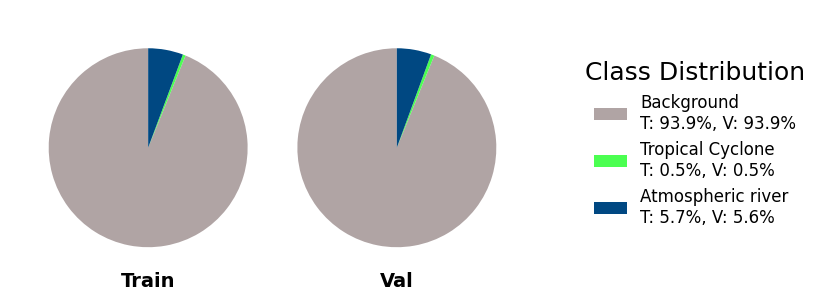
\includegraphics[width=1\textwidth]{graphics/background/data_distribution.png}
    \caption{Class Distribution}
    \label{fig:classdistribution}
\end{figure}


\begin{table}[h]
    \centering
    
    
    % Use p{width} for columns where you need wrapping text.
    \begin{tabular}{llccc}
        % \toprule
        \textbf{Type} & \textbf{Statistic} & \thead{\textbf{\#Masks} \\ \textbf{per Data Point}} & \thead{\textbf{Background/} \\ \textbf{Object } \\ \textbf{Per Mask}}  & \thead{\textbf{Background/} \\ \textbf{Object} \\ \textbf{per Data Point} } \\
        \midrule
        \multirow{2}{*}{\textbf{AR}}
            & Mean & 7.4 & 351.4 & 2,242 \\
            & Median & 7.0 & 142.2 & 17 \\
        \midrule
        \multirow{2}{*}{\textbf{TC}}
            & Mean & 2.6 & 880.7 & 149,220 \\
            & Median & 2.0 & 685.4 & 257 \\
        \bottomrule
    \end{tabular}
    \caption{Class Proportion and Object Statistics}
    \label{tab:summary_stats}
\end{table}






\subsection{Geographical Features and Constraint}
TCs are characterized by a distinct circular structure. Due to the lack of sufficient Coriolis force near the equator, these systems do not typically form within 5\degree{} of latitude. Instead, the vast majority of TCs originate within the latitudinal bands between 5\degree{} and 30\degree{} in both the Northern and Southern Hemispheres \cite{noaa_jetstream_tropical, hko_coriolis_tc}. Explainability analysis (LRP) confirms that CNNs indeed learn to look at point-shaped extrema in TMQ and circular wind motion to identify TCs \cite{radke2024explaining}.

ARs has narrow corridors or ``ribbons'' forms. These phenomena occur in both the Northern and Southern Hemispheres and are most commonly found in the mid-latitudes, typically between 30\degree{} and 60\degree{} \cite{gimeno2014atmospheric}. For AR detection, the models focus on elongated bands of high TMQ and eastward winds, which is physically plausible as ARs in both hemispheres are characterized by mid-latitude eastward moisture transport \cite{radke2024explaining}.

Consequently, when treating ClimateNet data points as spatial compositions, the geographic and geometric orientation of the corresponding labels is of critical importance. Because the formation of TCs and ARs are strictly governed by latitudinal physical constraints, the spatial context of these features is non-arbitrary. Therefore, standard geometric augmentation methods (e.g., vertical flipping or random rotations) should be avoided to ensure the model correctly learns the underlying geophysical semantics. Figure \ref{fig:world_projection_grid} illustrates four examples of data points from the ClimateNet dataset. As seen in these visualizations, the occurrence of these phenomena is variable; in some cases, TCs are not present within the provided time step, reflecting the natural distribution of extreme weather events.

% \begin{figure}[!h]
%     \centering
%     \begin{minipage}{0.48\textwidth}
%         \centering
%         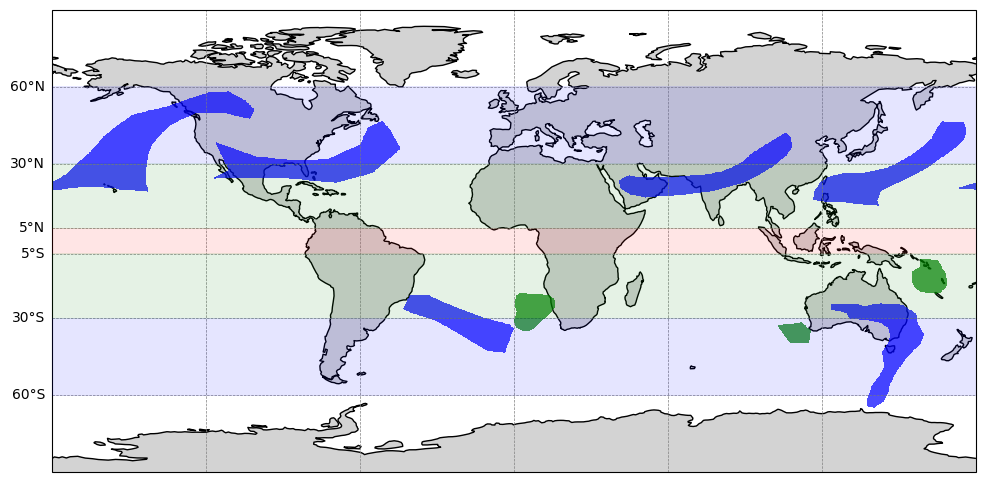
\includegraphics[width=1.05\textwidth]{graphics/background/data_example_1.png}
%         % \caption{a}
%     \end{minipage}
%     \hfill
%     \begin{minipage}{0.48\textwidth}
%         \centering
%         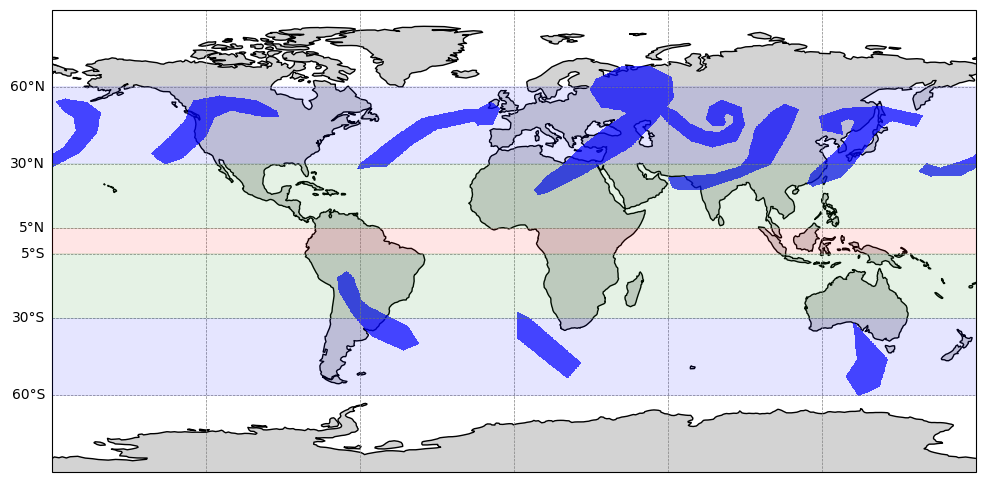
\includegraphics[width=1.05\textwidth]{graphics/background/data_example_2.png}
%         % \caption{b}
%     \end{minipage}
    
%     \vspace{0.5cm} % Add some vertical space
    
%     \begin{minipage}{0.48\textwidth}
%         \centering
%         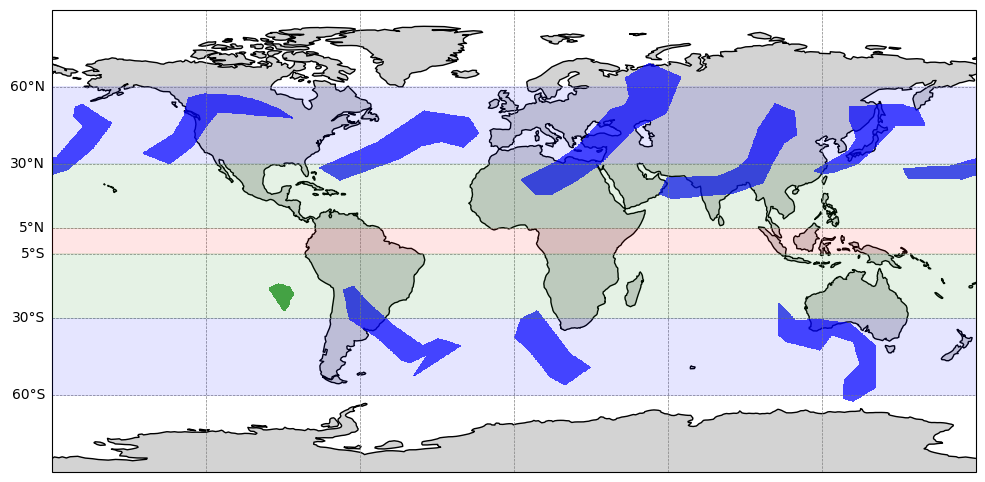
\includegraphics[width=1.05\textwidth]{graphics/background/data_example_3.png}
%         % \caption{c}
%     \end{minipage}
%     \hfill
%     \begin{minipage}{0.48\textwidth}
%         \centering
%         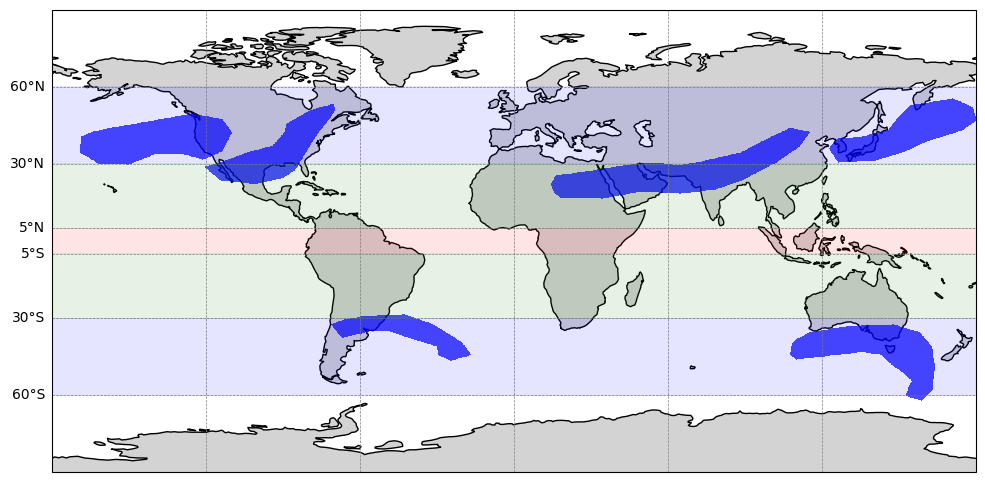
\includegraphics[width=1.05\textwidth]{graphics/background/data_example_4.png}
%         % \caption{d}
%     \end{minipage}
    
%     \caption{World projection visualizations of atmospheric data. The blue ``Ribons" are AR masks while, the green ones are TCs. The red band denotes the equatorial region between 5\degree{}N and 5\degree{}S where TCs do not typically form. The green bands (5\degree{} to 30\degree{} in both hemispheres) indicate the primary regions for TC activity. The purple bands (30\degree{} to 60\degree{} in both hemispheres) represent the mid\_latitudes where ARs typically occur.}
%     \label{fig:world_projection_grid}
% \end{figure}

\begin{figure}[!h]
    \centering
    \makebox[\textwidth][c]{%
        \begin{minipage}{1.0\textwidth}
            \centering
            \begin{minipage}{0.48\textwidth}
                \centering
                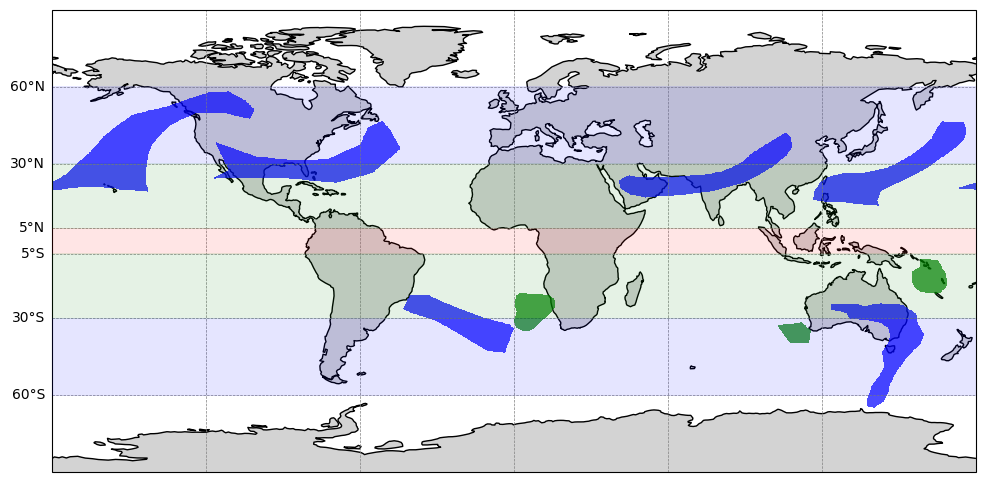
\includegraphics[width=1.05\textwidth]{graphics/background/data_example_1.png}
            \end{minipage}
            \hfill
            \begin{minipage}{0.48\textwidth}
                \centering
                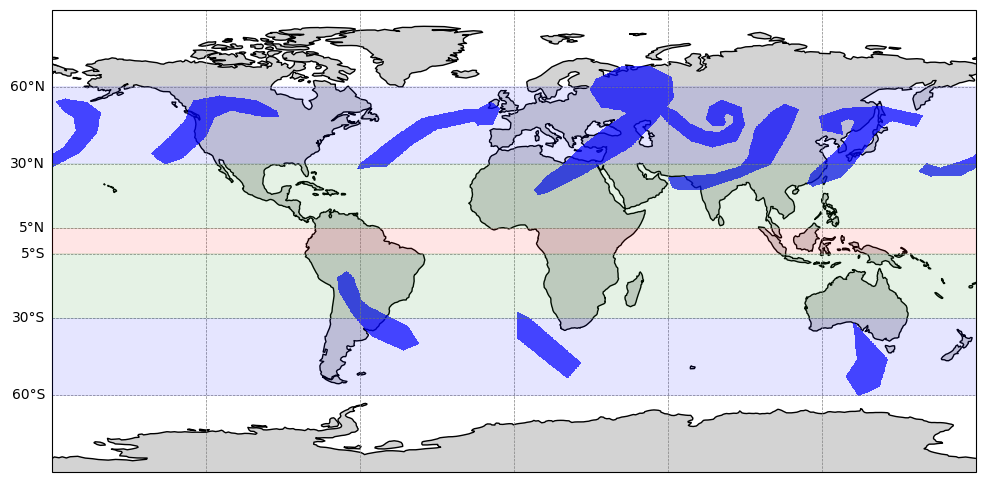
\includegraphics[width=1.05\textwidth]{graphics/background/data_example_2.png}
            \end{minipage}

            % \vspace{0.5cm}

            \begin{minipage}{0.48\textwidth}
                \centering
                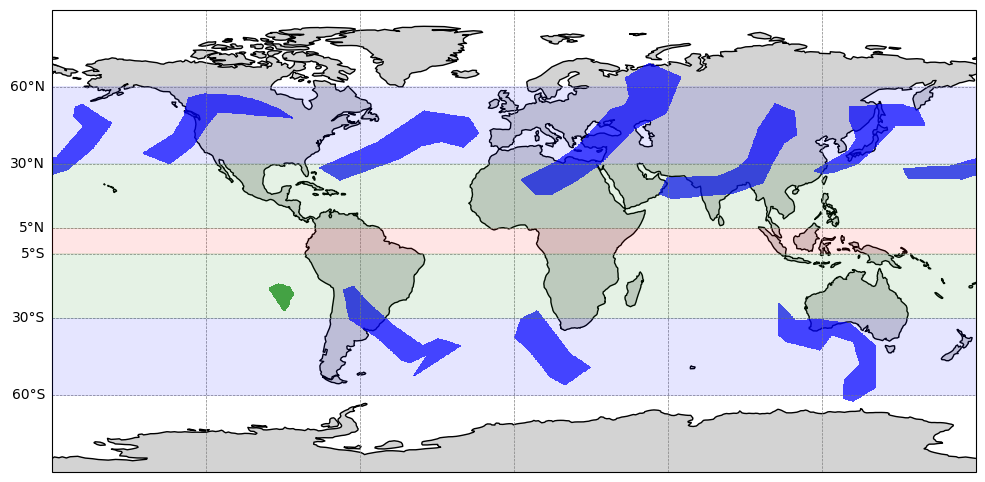
\includegraphics[width=1.05\textwidth]{graphics/background/data_example_3.png}
            \end{minipage}
            \hfill
            \begin{minipage}{0.48\textwidth}
                \centering
                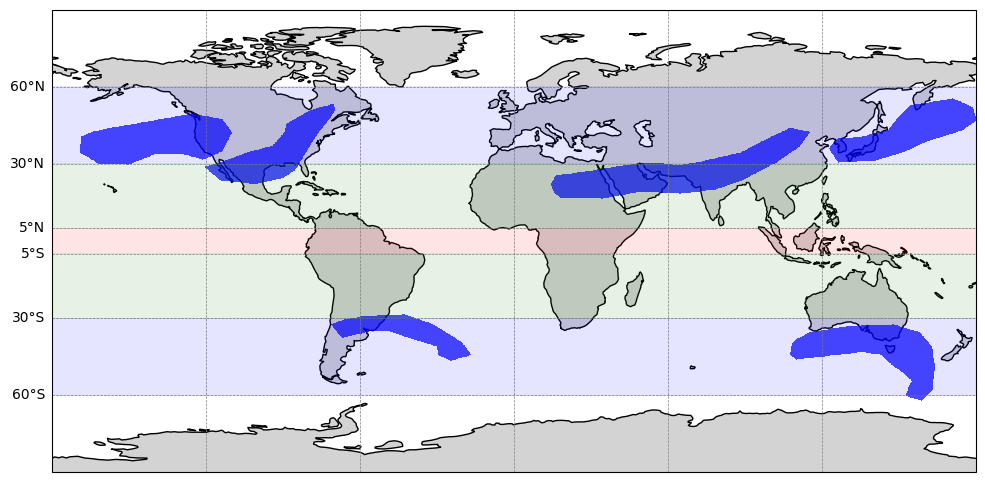
\includegraphics[width=1.05\textwidth]{graphics/background/data_example_4.png}
            \end{minipage}
        \end{minipage}
    }
    \caption{World projection visualizations of atmospheric data. The blue ``Ribons" are AR masks while, the green ones are TCs. The red band denotes the equatorial region between 5\degree{}N and 5\degree{}S where TCs do not typically form. The green bands (5\degree{} to 30\degree{} in both hemispheres) indicate the primary regions for TC activity. The purple bands (30\degree{} to 60\degree{} in both hemispheres) represent the mid\_latitudes where ARs typically occur.}
    \label{fig:data\_examples}
\end{figure}